\section{Results}
\label{sec:results}

The results begin with the multicity application outcome and then unpack
the evidence needed to interpret it. After the application overview, we
examine finite-sample behavior under known population conditions, report
the detailed city-level and local DELB estimates, evaluate them against
prespecified randomization references, assess sensitivity to spatial scale,
temporal aggregation, and sample size, and compare the estimated bounds
with held-out prediction errors. Table~\ref{tab:results_evidence_map}
summarizes the question addressed by each evidence layer.
Throughout this section, estimated CMI, changes in the estimated DELB,
randomization-calibrated information gain, and changes in realized
prediction error are treated as distinct empirical quantities.

\begin{table}[!t]
\begin{adjustwidth}{-\extralength}{0cm}
\caption{Evidence map for interpreting the empirical results. CMI denotes
conditional mutual information, and DELB denotes the Discrete Entropy Lower
Bound.}
\label{tab:results_evidence_map}
\scriptsize
\begin{tabularx}{\fulllength}{p{0.14\fulllength}XXX}
\toprule
\textbf{Evidence layer} & \textbf{Question answered} & \textbf{Main result} & \textbf{Interpretive boundary} \\
\midrule
City and local point estimates &
Does the estimated prediction floor decline after the bicycle state is added? &
Estimated conditional entropy and the corresponding DELB declined in all
cities and in the reported local summaries. &
Describes an estimated state-partition difference; it does not establish
bicycle-specific information. \\
Known-truth simulation and support diagnostics &
Can positive estimated CMI arise when population CMI is zero? &
Sparse nested states produced positive plug-in and Miller--Madow estimates
and nonzero randomization centers; support complexity tracked both behaviors. &
Diagnoses finite-sample estimation and calibration, not the city-specific
mobility effect. \\
Randomization and multiscale calibration &
Is the observed statistic unusually large under prespecified null mechanisms? &
No primary or multiscale comparison survived the relevant calibration and
multiplicity correction. &
Limits attribution to recent, geographically matched bicycle mobility; it
does not prove conditional independence. \\
Matched prediction and Predictability Gap &
Did fitted models convert the augmented state into lower held-out MSE? &
Improvements were model- and city-dependent, and only two New York models
narrowed the estimated gap. &
Realized model performance neither proves nor refutes a population DELB
change. \\
Fano comparison &
Does the information ordering persist under classification loss? &
Estimated Fano floors declined, while sparse held-out modal classifiers often
worsened. &
Fano and DELB use different targets and losses; their magnitudes are not
directly comparable. \\
Heterogeneity and robustness &
Does the descriptive pattern depend on target or specification? &
Positive DELB-reduction point estimates were widespread, whereas predictive
improvements remained heterogeneous. &
Changed targets and units preclude direct effect-size comparisons; category
results are exploratory. \\
\bottomrule
\end{tabularx}
\end{adjustwidth}
\end{table}

\subsection{Multicity Application Results at a Glance}
\label{subsec:application_results_overview}

\begin{table}[!htbp]
\caption{Application-level synthesis across the three cities. The
transformation-reference column reports the smallest unadjusted \(p\)-value
across the temporal-block, spatial-series, and circular-shift references; the
matched-reference column reports the \(p\)-value from baseline-state-matched
restricted randomization. Positive prediction screens are adjusted within
the matched city--model comparisons.}
\label{tab:application_results_overview}
\centering
\setlength{\tabcolsep}{2pt}
\begin{tabular*}{\textwidth}{@{\extracolsep{\fill}}lrrrrrr@{}}
\toprule
\textbf{City} & \shortstack{\textbf{Complete-domain}\\\(\boldsymbol{\Delta L}\)} &
\shortstack{\textbf{Covered}\\\(\boldsymbol{\Delta L}\)} &
\shortstack{\textbf{Covered relative}\\\textbf{reduction}} &
\shortstack{\textbf{Transform.}\\\textbf{min. \(p\)}} &
\shortstack{\textbf{Matched}\\\(\boldsymbol{p}\)} &
\shortstack{\textbf{Positive screens /}\\\textbf{gap narrowing}}\\
\midrule
Washington, DC & 0.0119 & 0.0123 & 7.9\% & 0.967 & 0.599 & 0/4 \quad / \quad 0/4\\
New York City & 0.0094 & 0.0604 & 17.3\% & 0.986 & 0.999 & 2/4 \quad / \quad 2/4\\
Vancouver & 0.0115 & 0.0919 & 18.0\% & 0.903 & 0.994 & 1/4 \quad / \quad 0/4\\
\bottomrule
\end{tabular*}
\end{table}


The application produced a consistent descriptive ordering but not a
consistent inferential or predictive gain
(Table~\ref{tab:application_results_overview}). Within the
bicycle-covered populations, adding lagged bicycle flow reduced the
estimated DELB by 7.9\% in Washington, DC, 17.3\% in New York City, and
18.0\% in Vancouver. The reductions remained positive in the complete
crime-supported populations, although they attenuated sharply in New York
City and Vancouver.

Neither the three E10 transformation references nor the E18
baseline-state-matched reference separated the observed CMI in any city.
Held-out prediction was also selective: adjusted positive-improvement
screens occurred for two of four New York models and one Vancouver model,
whereas only the two New York models narrowed the estimated Predictability
Gap. Thus, the direct application result is not that bicycle mobility
uniformly improves crime prediction. It is that a positive estimated
information-floor change can coexist with non-rejection under calibrated
references and model-dependent realized performance. The following
subsections provide the finite-sample and experiment-specific evidence
behind that synthesis.

\subsection{Finite-Sample Behavior of CMI Estimation}
\label{subsec:results_e12_simulation}

Known-truth simulations were examined before the urban estimates to
determine how sparse nested states affect CMI estimation and
transformation-based calibration. Population CMI was obtained
by exact enumeration, so estimator bias could be separated from the
center of the corresponding randomization distribution.

Under the 72 population-null design cells, both estimators produced
positive CMI estimates despite the true CMI being zero. Mean null bias
was \SimPluginNullBias{} bits for the plug-in estimator and \SimMMNullBias{} bits
for the Miller--Madow estimator. Increasing the sample size from 365 to 1095
observations reduced average bias, whereas larger joint state spaces,
greater singleton occupancy, and larger effective conditional degrees
of freedom increased it. The Miller--Madow correction reduced average
bias but did not uniformly outperform the plug-in estimator in the
sparsest designs.

The transformation-specific reference distributions were also positively centered.
Their mean centers were \SimPluginNullCenter{} bits for the plug-in estimator
and \SimMMNullCenter{} bits for the Miller--Madow estimator. Despite these nonzero centers,
the mean Type I rejection rates were \SimPluginTypeI{} and \SimMMTypeI{},
respectively, because the observed statistics were compared with their
complete transformation-specific reference distributions rather than with
zero. Mean power across the positive-CMI designs was \SimPluginPower{} for
the plug-in estimator and \SimMMPower{} for the Miller--Madow estimator (Table~\ref{tab:e12_simulation_summary}
and Figure~\ref{fig:e12_sparse_simulation}).

\begin{table}[!htbp]
\caption{Finite-sample CMI simulation summary. Null bias and null centers are in bits. Size is the mean rejection rate under population CMI equal to zero; power averages the positive-CMI designs.}
\label{tab:e12_simulation_summary}
\centering
\begin{tabular*}{\textwidth}{@{\extracolsep{\fill}}lcccc@{}}
\toprule
\textbf{Estimator} & \textbf{Mean null bias} & \textbf{Mean null center} & \textbf{Size} & \textbf{Power}\\
\midrule
Plug-in & 0.1651 & 0.2069 & 0.014 & 0.337\\
Miller--Madow & 0.1264 & 0.1376 & 0.011 & 0.447\\
\bottomrule
\end{tabular*}
\end{table}


\begin{figure}[H]
\begin{adjustwidth}{-\extralength}{0cm}
\centering
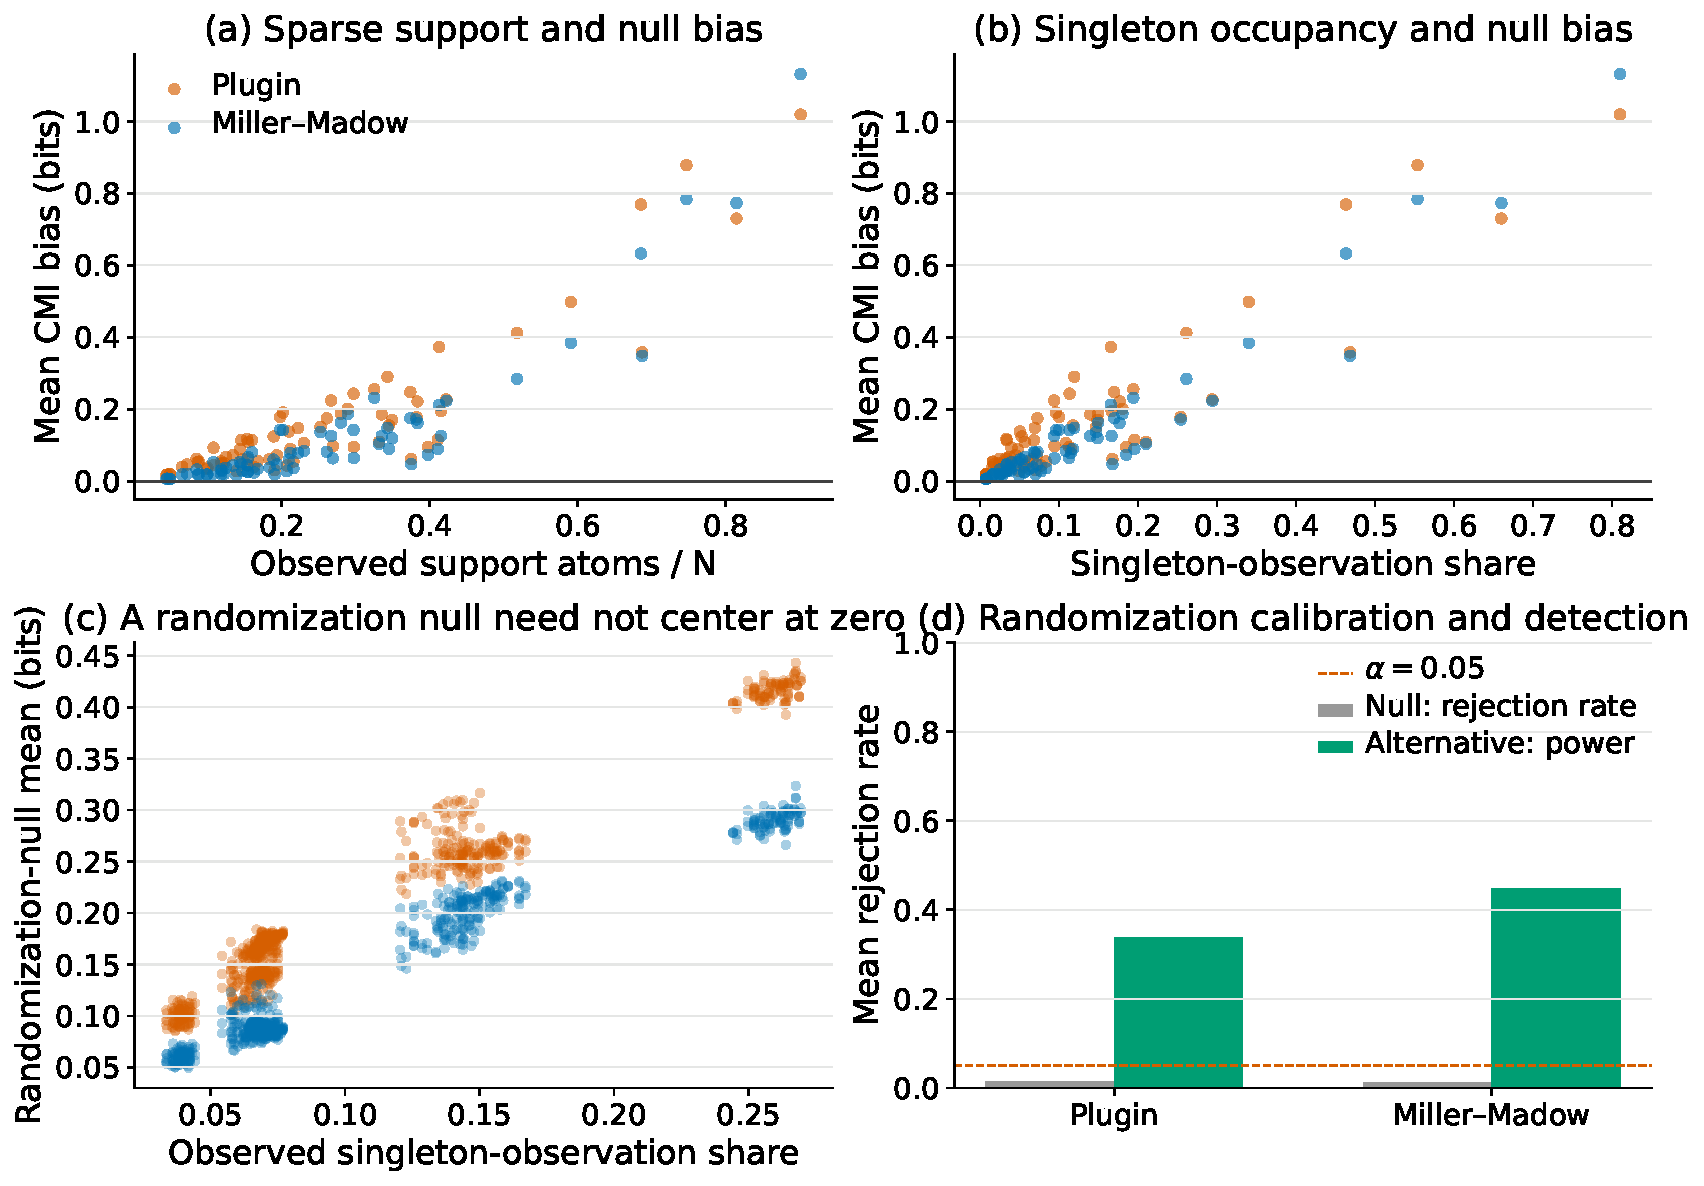
\includegraphics[width=\linewidth]{figures/s7/e12_sparse_cmi_main.pdf}
\end{adjustwidth}
\caption{Known-truth simulation of sparse nested-state CMI estimation and
randomization behavior. Population CMI is obtained by exact enumeration.
Positive estimator bias and a positive randomization center are distinct
finite-sample objects.}
\label{fig:e12_sparse_simulation}
\end{figure}

Support diagnostics showed consistent associations with finite-sample
behavior. In the known-null simulations, observed-atom density,
singleton-observation share, and normalized effective degrees of freedom
were associated with the bias of both estimators. Across the 1017 empirical
city--grid--reference summaries, their Spearman correlations with the
randomization-reference mean were 0.835, 0.866, and 0.988, respectively.
In a fixed-effects model with city-grid-clustered standard errors,
surrogate normalized effective degrees of freedom had a coefficient of
\SupportCombinedNuCoefficient{} (SE \SupportCombinedNuSE{};
\(R^2=\SupportCombinedNullRSquared{}\)).

The transformations also changed the CMI support.
Changes in support complexity between each surrogate and the observed
table were negatively associated with observed-minus-reference CMI, with correlations ranging
from \(-0.653\) to \(-0.791\). These relations are diagnostic rather than
causal and do not define a universal bias correction. They show that the
center of a finite-sample randomization distribution depends jointly on
the estimator, observed support, and transformation design. Accordingly,
the city analyses below compare observed CMI with complete design-matched
reference distributions rather than using zero as an automatic benchmark.



\begin{table}[H]
\caption{Association of support diagnostics with CMI estimator behavior. Entries are Spearman correlations. The first two columns use population-null simulations; the last two use 1,017 city-grid-null summaries.}
\label{tab:e13_support_relationships}
\begin{adjustwidth}{-\extralength}{0cm}
\centering
\small
\begin{tabular}{lrrrr}
\toprule
\textbf{Metric} & \textbf{Plugin bias} & \textbf{MM bias} & \textbf{Null mean} & \textbf{Observed--null}\\
\midrule
$K_{\mathrm{obs}}/N$ & 0.840 & 0.891 & 0.835 & -0.653\\
$S_1$ & 0.819 & 0.909 & 0.866 & -0.656\\
$\nu/N$ & 0.989 & 0.950 & 0.988 & -0.791\\
\bottomrule
\end{tabular}
\end{adjustwidth}
\end{table}


\begin{figure}[H]
\begin{adjustwidth}{-\extralength}{0cm}
\centering
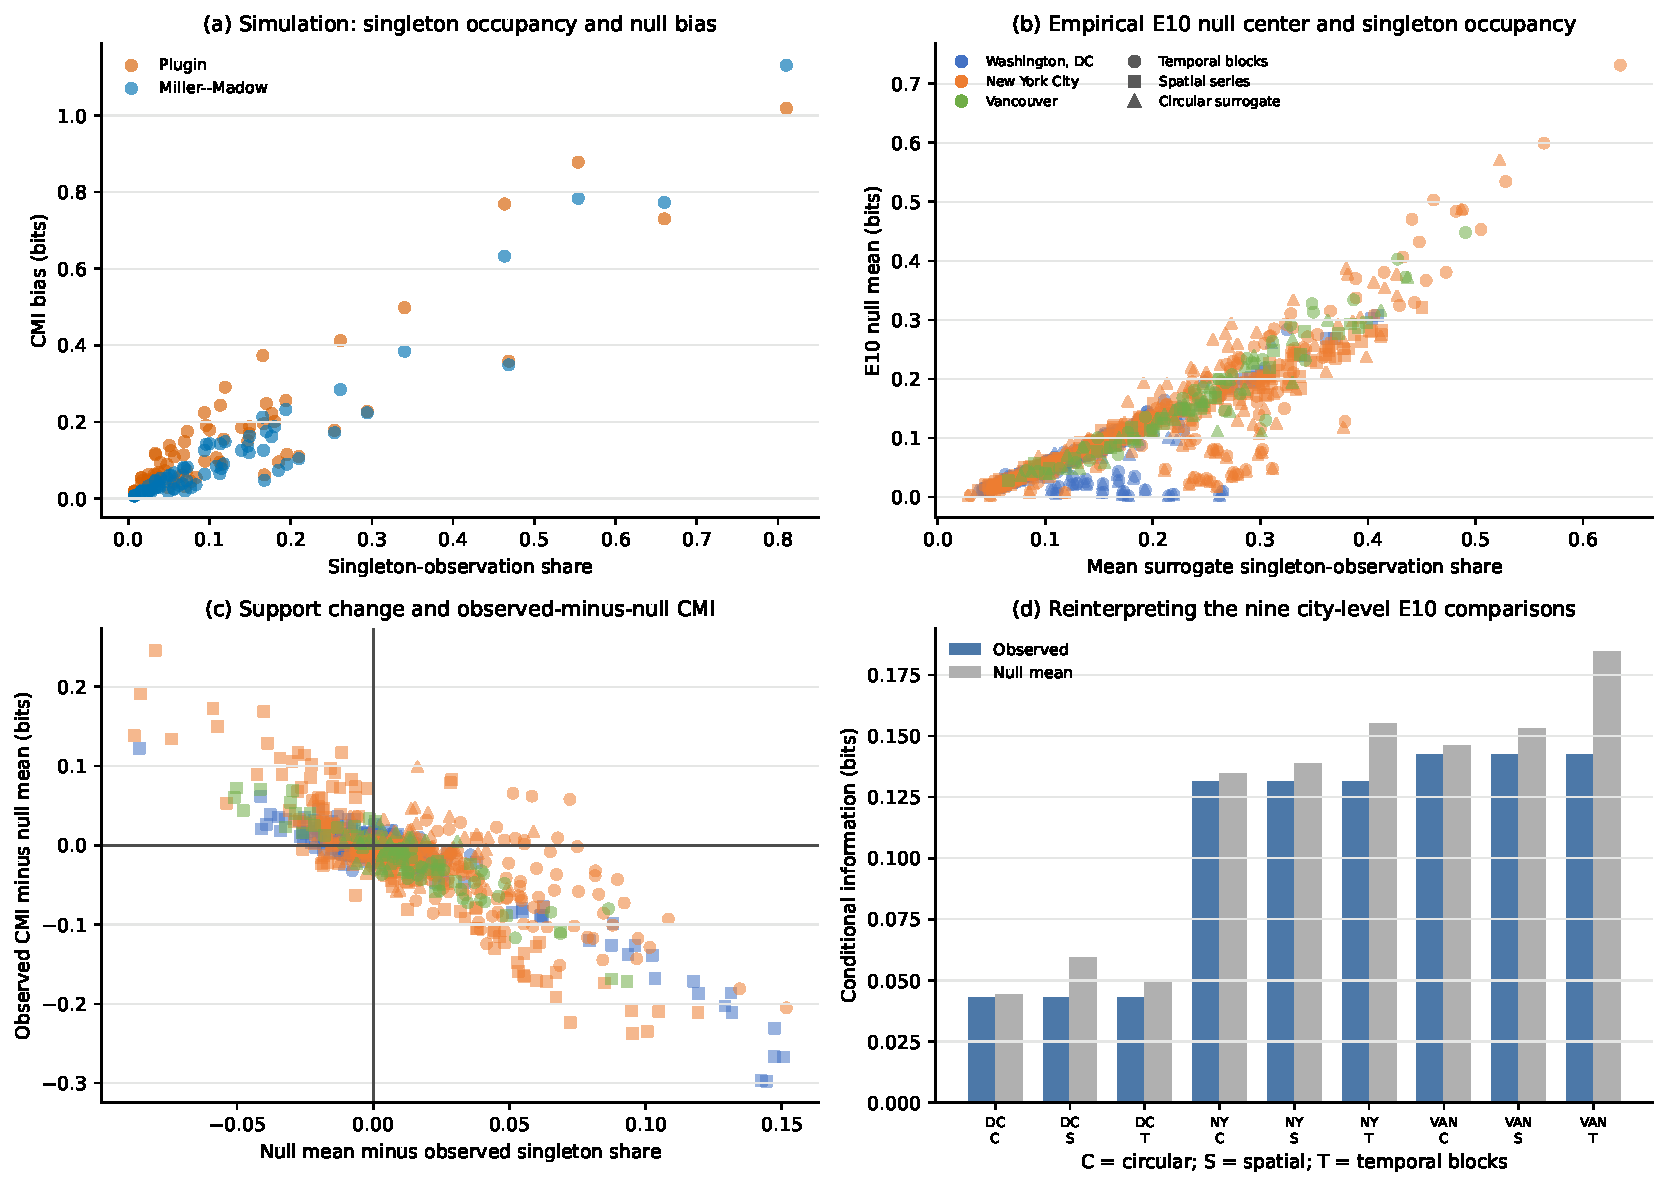
\includegraphics[width=\linewidth]{figures/s7/e13_support_null_main.pdf}
\end{adjustwidth}
\caption{Support structure and randomization-reference centering. Simulation
panels use known zero population CMI; empirical panels use
surrogate-specific support recomputed after every transformation. Lines are
descriptive associations.}
\label{fig:e13_support_null}
\end{figure}

\subsection{Estimated City-Level and Local Prediction Bounds}
\label{subsec:results_city_information}

At the pooled city level, adding the one-day-lagged bicycle state reduced
estimated conditional entropy in all three cities. The Miller--Madow CMI
estimates were \DCCMI{} bits in Washington, DC,\NYCMI{} bits in New York, and \VANCMI{} bits in Vancouver.
Mapping the baseline and bicycle-augmented conditional entropies through the
same inverse integer-lattice envelope produced estimated DELB reductions of
\DCDeltaL{} MSE units in Washington, DC, \NYDeltaL{} in New York City, and
\VANDeltaL{} in Vancouver. These changes represented relative reductions of
\DCRelativeL, \NYRelativeL, and \VANRelativeL, respectively
(Table~\ref{tab:city_entropy_results} and
Figure~\ref{fig:city_information_bounds}).
The centered seven-day block-bootstrap intervals for the CMI estimates
excluded zero. These intervals quantify sampling variation under the
observed state partition and dependence structure; randomization-based
attribution is examined separately in Section~\ref{subsec:results_nulls}.



\begin{table}[H]
\caption{Pooled city-level conditional entropy and DELB results in the training bicycle-covered domain. Brackets report centered 95\% seven-day block-bootstrap intervals for CMI.}
\label{tab:city_entropy_results}
\begin{adjustwidth}{-\extralength}{0cm}
\centering
\begin{tabular*}{\linewidth}{@{\extracolsep{\fill}}lrrrrrrrr@{}}
\toprule
\textbf{City} & \(\boldsymbol{N}\) & \(\boldsymbol{H^0}\) &
\(\boldsymbol{H^B}\) & \textbf{CMI [95\% CI]} &
\(\boldsymbol{L^0}\) & \(\boldsymbol{L^B}\) &
\(\boldsymbol{\Delta L}\) & \(\boldsymbol{R^L}\)\\
\midrule
Washington, DC & 198,195 & 0.783 & 0.740 & 0.043 [0.040, 0.047] & 0.157 & 0.144 & 0.012 & 7.9\%\\
New York City & 216,810 & 1.293 & 1.162 & 0.131 [0.123, 0.140] & 0.350 & 0.290 & 0.060 & 17.3\%\\
Vancouver & 37,230 & 1.563 & 1.421 & 0.142 [0.126, 0.159] & 0.511 & 0.419 & 0.092 & 18.0\%\\
\bottomrule
\end{tabular*}
\end{adjustwidth}
\end{table}


\begin{figure}[!t]
\centering
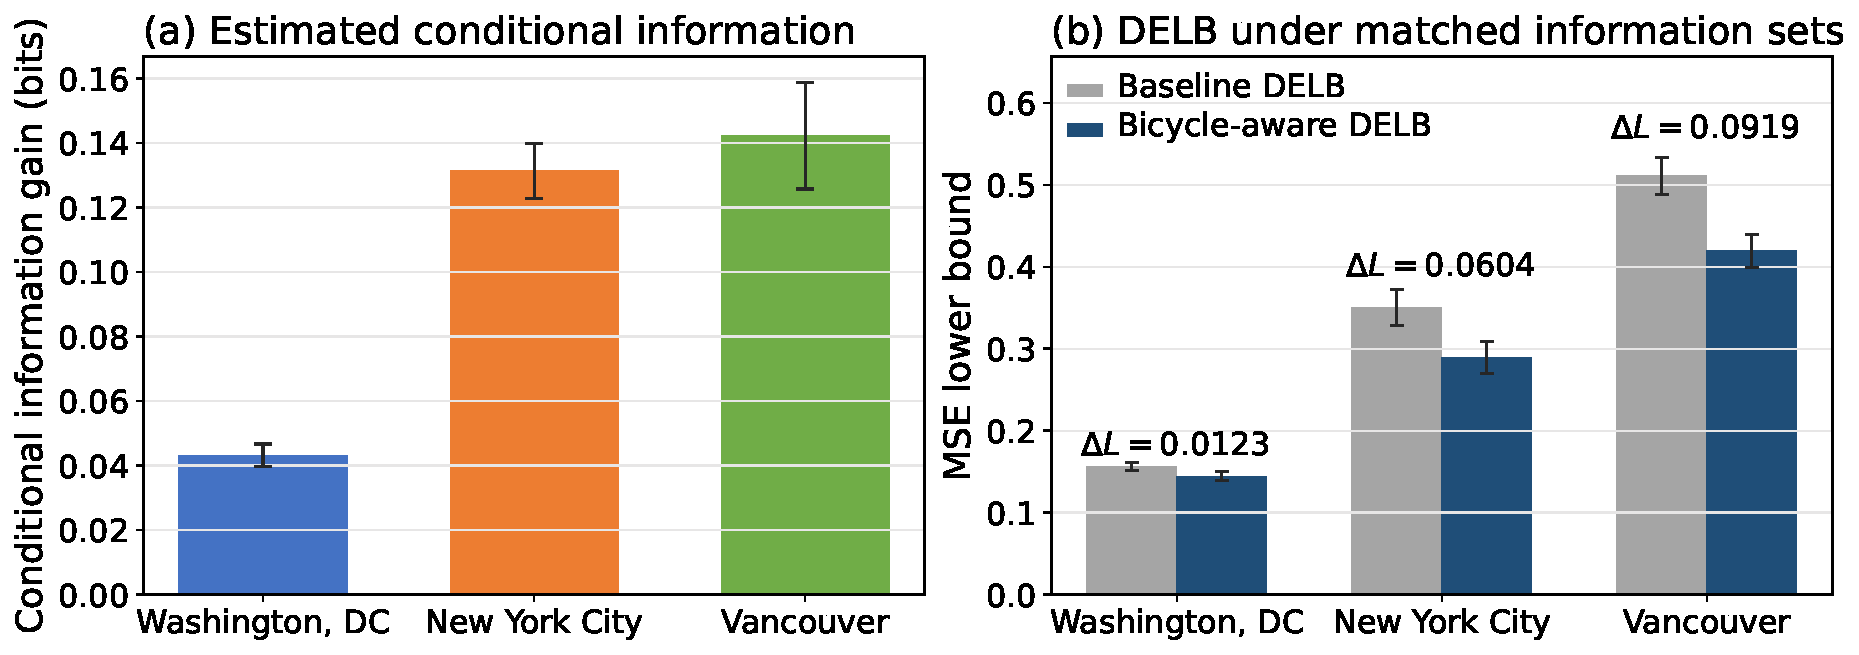
\includegraphics[width=\textwidth]{figures/e17/e17_city_cmi_delb_combined.pdf}
\caption{Primary city-level point estimates. \textbf{(a)} Miller--Madow CMI
with centered 95\% seven-day block-bootstrap intervals.
\textbf{(b)} DELB-implied MSE floors under the baseline and bicycle-aware
information sets. These intervals describe sampling variation under the
observed support; randomization calibration is reported in
Section~\ref{subsec:results_nulls}.}
\label{fig:city_information_bounds}
\end{figure}
\FloatBarrier

\begin{table}[!htbp]
\caption{City-level DELB point estimates for two training-period-frozen
analysis populations. The deployment population uses the complete
crime-supported domain; the bicycle-covered population uses its
bicycle-covered subset.}
\label{tab:co_primary_domains}
\begin{adjustwidth}{-\extralength}{0cm}
\centering
\begin{tabular*}{\linewidth}{@{\extracolsep{\fill}}llrrrrrr@{}}
\toprule
\textbf{City} & \textbf{Population} & \textbf{Grids} & \textbf{\(N\)} &
\textbf{CMI (bit)} & \textbf{\(L^0\)} & \textbf{\(L^B\)} &
\textbf{\(\Delta L\)}\\
\midrule
Washington, DC & Deployment (complete) & 186 & 203,670 & 0.0420 & 0.1535 & 0.1416 & 0.0119\\
Washington, DC & Coverage-conditioned & 181 & 198,195 & 0.0432 & 0.1567 & 0.1443 & 0.0123\\
New York City & Deployment (complete) & 806 & 882,570 & 0.0348 & 0.1382 & 0.1288 & 0.0094\\
New York City & Coverage-conditioned & 198 & 216,810 & 0.1314 & 0.3503 & 0.2898 & 0.0604\\
Vancouver & Deployment (complete) & 141 & 154,395 & 0.0377 & 0.1774 & 0.1659 & 0.0115\\
Vancouver & Coverage-conditioned & 34 & 37,230 & 0.1423 & 0.5113 & 0.4194 & 0.0919\\
\bottomrule
\end{tabular*}
\end{adjustwidth}
\end{table}


The two co-primary, training-period-frozen populations retained positive
city-level point estimates (Table~\ref{tab:co_primary_domains}). In the complete
crime-supported domain, CMI was 0.0420, 0.0348, and 0.0377 bits in
Washington, DC, New York City, and Vancouver, respectively, compared with
0.0432, 0.1314, and 0.1423 bits in the bicycle-covered domain. The
corresponding complete-domain DELB reductions were 0.0119, 0.0094, and
0.0115 MSE units, versus 0.0123, 0.0604, and 0.0919. Thus, the sign was
stable, but the magnitude in New York City and Vancouver depended strongly
on the spatial target population. This co-primary comparison concerns
city-level point estimates only; the downstream inferential experiments
retain their prespecified bicycle-covered populations.

\subsubsection{Local Estimates and Spatial Patterning}
\label{subsec:results_local_information}

Of 413 bicycle-covered cells, 339 met local eligibility criteria: 146 in
Washington, DC, 160 in New York, and 33 in Vancouver. Median local DELB
reductions were \DCLocalMedianDeltaL{}, \NYLocalMedianDeltaL{}, and
\VANLocalMedianDeltaL{} units, respectively.The sampling-uncertainty screen
was positive in 137 of 146 Washington cells, 155 of 160 New York cells,
and all 33 eligible Vancouver cells.

Spatial autocorrelation differed across cities. Global Moran's \(I\) for
the local DELB reduction was 0.164 in Washington, DC (\(p=0.002\)), 0.038 in New York City
(\(p=0.261\)), and 0.171 in Vancouver (\(p=0.022\)). Thus, local point
estimates were spatially clustered in Washington and Vancouver but not
detectably clustered in New York under the specified contiguity design.

The local table and map are reported in Supplementary Materials, Section S2.
Their colors represent
point-estimate magnitude rather than statistical significance; the
randomization analysis below evaluates whether the observed local
reductions exceed their temporal, spatial, and circular-shift references.

\subsection{Randomization Calibration and Lag Specificity}
\label{subsec:results_nulls}

The randomization analyses evaluated whether the observed CMI was unusually
large relative to three prespecified transformation-based reference
distributions. Evidence under a given design required the observed
statistic to fall in the upper tail of that reference distribution;
the reference center was not constrained to zero.

None of the nine city-by-reference comparisons rejected its corresponding
upper-tail null. Unadjusted \(p\)-value ranged from 0.903 to 1.000, and all multiplicity-adjusted
\(q\)-value were 1.000. In most comparisons, the observed CMI was below
the corresponding reference mean. At the local level, none of the 339
eligible cells passed all three randomization designs, including cells
that had passed the block-bootstrap sampling-uncertainty screen.

E17 produced the same city-level conclusion for all three entropy
estimators. Across the nine comparisons within each estimator, raw
\(p\)-values ranged from 0.980 to 1.000 for plug-in, 0.903 to 1.000 for
Miller--Madow, and 0.984 to 1.000 for Jeffreys--Dirichlet. No comparison
passed either the estimator-specific nine-test correction
(\ESeventeenWithinRejects{}/27) or the global 27-test correction
(\ESeventeenGlobalRejects{}/27). The full estimator-specific null summaries
are reported in Supplementary Materials, Section S1.

The distant-lag analysis produced similar CMI estimates. Ratios of
14-day- or 30-day-lag CMI to the matched one-day-lag CMI ranged from
\DistantRatioMin{} to \DistantRatioMax{}. Both distant-lag estimates
exceeded the one-day estimate in New York City, whereas differences
in Washington, DC and Vancouver were small and inconsistent
(Table~\ref{tab:null_calibration}). The detailed lag figure is retained in
Supplementary Materials, Section S2.

Taken together, the three randomization designs and distant-lag comparisons
did not isolate an information signal specific to recent, geographically
matched bicycle activity. The results nevertheless remain conditional on
the transformations examined; they do not constitute a general test of
conditional independence.

\begin{table}[!htbp]
\caption{Baseline-state-matched restricted randomization and semi-synthetic
calibration. Type I error and power use 50 Monte Carlo datasets and 99
randomizations per dataset under the fitted-dispersion scenario.}
\label{tab:e18_restricted_calibration}
\centering
\setlength{\tabcolsep}{2.5pt}
\begin{tabular*}{\textwidth}{@{\extracolsep{\fill}}lrrrrrrr@{}}
\toprule
\textbf{City} & \shortstack{\textbf{Observed}\\\textbf{CMI}} &
\shortstack{\textbf{Null}\\\textbf{mean}} &
\textbf{\(p\)} & \shortstack{\textbf{Type I}\\\textbf{error}} &
\shortstack{\textbf{Power at}\\\textbf{0.02 bit}} &
\shortstack{\textbf{Power at}\\\textbf{0.05 bit}} &
\shortstack{\textbf{Power at highest}\\\textbf{evaluated CMI}}\\
\midrule
Washington, DC & 0.0432 & 0.0433 & 0.599 & 0.04 & 0.10 & 0.06 &
0.48 at 0.0649 bit\\
New York City & 0.1314 & 0.1338 & 0.999 & 0.08 & 0.02 & 0.02 &
0.46 at 0.1000 bit\\
Vancouver & 0.1423 & 0.1476 & 0.994 & 0.00 & 0.02 & 0.02 &
0.30 at 0.1000 bit\\
\bottomrule
\end{tabular*}
\end{table}


The baseline-state-matched restricted randomization reached a movable-block
share of 1.00 in every city and preserved the bicycle-state marginal
exactly. Its null means were again slightly above the observed CMI
(Table~\ref{tab:e18_restricted_calibration}). The upper-tail \(p\)-values
were 0.599, 0.999, and 0.994 in Washington, DC, New York City, and
Vancouver; all three BH-adjusted \(q\)-values were 0.999. Thus, bringing
the reference closer to the baseline state did not reverse the E10
non-rejection.

The semi-synthetic results qualified that finding. Under zero population
CMI, restricted-design rejection rates ranged from 0.00 to 0.08 across
cities and dispersion settings, and every exact 95\% binomial interval
covered 0.05. However, power at 0.02 and 0.05 bit was only 0.00--0.10.
Even under the fitted-dispersion scenario, power at the highest evaluated
attainable CMI was 0.48 in Washington, DC, 0.46 in New York City, and
0.30 in Vancouver. Some requested high-CMI settings were unattainable on
the fixed empirical support and were reported at their actual maxima.
Consequently, E18 supports calibration of the restricted reference but
also shows limited detection power; its non-rejection cannot establish
conditional irrelevance.




\begin{table}[H]
\caption{\rev{Randomization-reference calibration and distant-lag diagnostics.} Randomization
\(p\)-values are upper-tail tests of whether observed CMI exceeds the
specified null distribution. Distant-lag columns report
\(\widehat I_{\mathrm{distant}}/\widehat I_{\mathrm{recent}}\).}
\label{tab:null_calibration}
\centering
\begin{tabular*}{\linewidth}{@{\extracolsep{\fill}}lrrrrr@{}}
\toprule
\textbf{City} & \multicolumn{3}{c}{\textbf{Randomization \(p\)-value}} &
\multicolumn{2}{c}{\textbf{Distant/recent CMI}}\\
\cmidrule(lr){2-4}\cmidrule(lr){5-6}
 & \textbf{Temporal} & \textbf{Spatial} & \textbf{Circular} &
\textbf{14 days} & \textbf{30 days}\\
\midrule
Washington, DC & 1.000 & 1.000 & 0.967 & 0.992 & 0.985\\
New York City & 1.000 & 0.986 & 0.993 & 1.020 & 1.052\\
Vancouver & 1.000 & 0.969 & 0.903 & 0.964 & 1.007\\
\bottomrule
\end{tabular*}
\end{table}


\begin{figure}[!t]
\begin{adjustwidth}{-\extralength}{0cm}
\centering
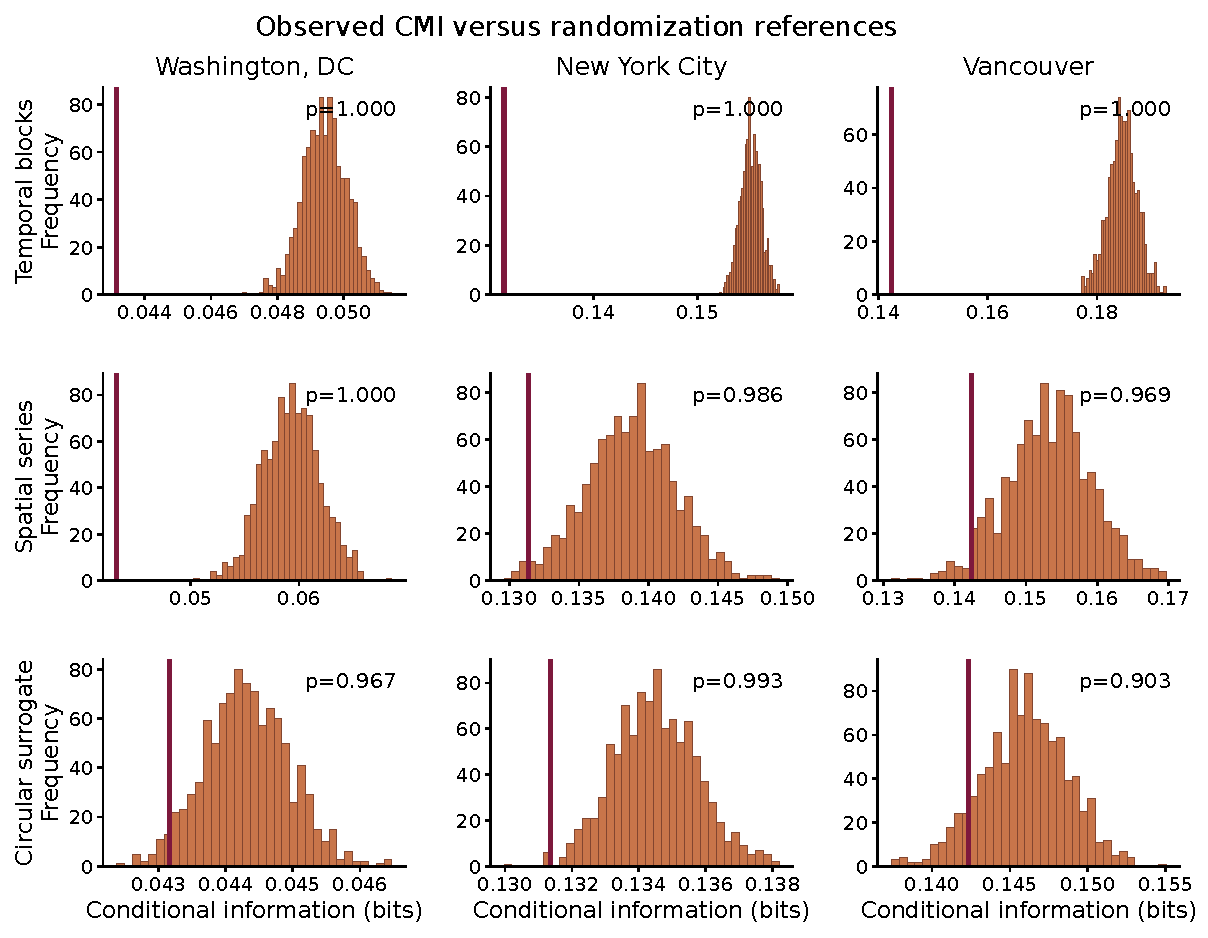
\includegraphics[width=\linewidth]{figures/e11/e10_city_null_distributions.pdf}
\end{adjustwidth}
\caption{Observed city-level CMI relative to temporal-block,
spatial-series, and circular-shift reference distributions. The observed
statistic did not exceed any prespecified upper-tail reference.}
\label{fig:city_nulls}
\end{figure}



\subsection{Spatiotemporal Scale and Sample-Size Calibration}
\label{subsec:e16_scale_results}

The multiscale analysis separated three sources of variation. Spatial
and temporal aggregation changed the prediction target, sample thinning
evaluated estimator stability within a fixed design, and randomization
compared each observed statistic with its transformation-specific reference.

Across the 18 full-sample city--space--time combinations, estimated
Miller--Madow CMI ranged from \ScaleFullCMIMin{} to \ScaleFullCMIMax{} bits,
and singleton-observation share ranged from \ScaleSingletonMin{} to \ScaleSingletonMax{}.
Every full-sample combination produced a positive estimated DELB reduction.
After deterministic area--time scaling, reductions in the implied RMSE floor
ranged from \ScaleIntensityReductionMin{} to \ScaleIntensityReductionMax{} crimes
km\(^{-2}\) day\(^{-1}\). Because aggregation changes both the outcome
distribution and the MSE unit, these values describe distinct
scale-specific targets rather than repeated estimates of one
scale-invariant quantity.

Estimator stability improved as more time blocks were retained. At the 20\%
sample fraction, the median relative deviations from the corresponding full-sample estimates
were \ScaleBoundStabilityTwenty{} for the baseline DELB, 0.646 for the
bicycle-aware DELB, 0.630 for the DELB reduction, and \ScaleCMIStabilityTwenty{} for CMI.
At the 80%
fraction, these deviations had declined to \ScaleBoundStabilityEighty{}, 0.114,
0.070 and \ScaleCMIStabilityEighty{}, respectively
(Supplementary Materials, Section S3).
These deviations measure agreement with the full-sample estimate
rather than distance from the unknown population quantity.

Randomization results were consistent across scales and sample fractions.
None of the 270 city--space--time--sample--reference tests survived either the
global or within-family FDR correction. The minimum unadjusted \(p\)-value was
\ScaleMinimumRawP{} and the minimum within-family \(q\)-value was
\ScaleMinimumWithinQ{}.
Thirty-three observed CMI values exceeded their corresponding reference
means, but none did so under temporal-block randomization.
At the prespecified full-sample scales, the New York 500 m
daily circular-shift comparison had \(p=0.006\), but its global
\(q\)-value was \(q=0.54\).

Thus, positive estimated DELB reductions occurred at every full-sample
scale, while the prespecified multiscale calibration produced no
multiplicity-adjusted evidence that the reductions were specific
to the aligned bicycle state.


\begin{table}[H]
\caption{Multiscale upper-tail randomization calibration. Discoveries use a Benjamini--Hochberg adjustment across all 270 tests.}
\label{tab:e16_randomization_summary}
\begin{adjustwidth}{-\extralength}{0cm}
\centering
\small
\begin{tabular}{lccccc}
\toprule
\textbf{Null design} & \textbf{Tests} & \textbf{Min. $p$} & \textbf{Median $p$} & \textbf{Obs. $>$ null} & \textbf{FDR discoveries}\\
\midrule
Temporal block & 90 & 0.873 & 1.000 & 0 & 0\\
Spatial series & 90 & 0.130 & 0.945 & 12 & 0\\
Circular shift & 90 & 0.005 & 0.917 & 21 & 0\\
\bottomrule
\end{tabular}
\end{adjustwidth}
\end{table}


\begin{figure}[H]
\begin{adjustwidth}{-\extralength}{0cm}
\centering
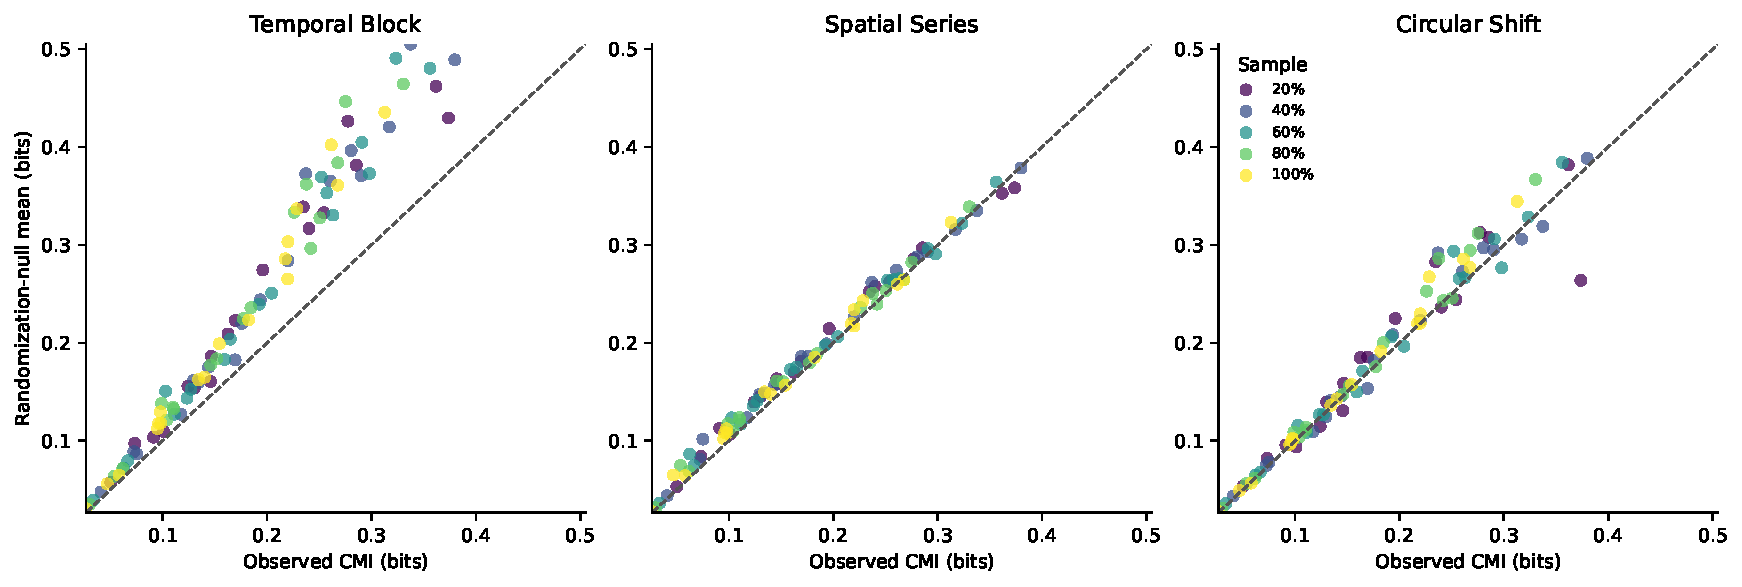
\includegraphics[width=\linewidth]{figures/e16/e16_s16_6_observed_vs_null.pdf}
\end{adjustwidth}
\caption{Observed Miller--Madow CMI versus the randomization-reference mean
across 270 city--space--time--sample--design comparisons. The dashed line is
equality; a nonzero reference center is allowed and is not population CMI.}
\label{fig:e16_observed_null}
\end{figure}


\subsection{Held-Out Prediction and Predictability Gaps}
\label{subsec:results_prediction}

Held-out prediction evaluated whether particular fitted models converted
the augmented information state into lower error on unseen observations.
The fixed July--December 2022 test set contained 75,992 grid--day observations.

Adding the bicycle state reduced the MSE point estimate in six of the 12
city--model comparisons. Three comparisons passed the adjusted
positive-improvement screen: the state-mean and Poisson gradient-boosting
models in New York City and the state-mean model in Vancouver.
The remaining model--city combinations showed either negligible change
or higher MSE after the bicycle state was added (Figure~\ref{fig:mse_improvement}).

All held-out MSE values remained above their matched DELB estimates.
The New York state-mean model narrowed the estimated Predictability Gap
by 0.001 MSE units, and New York gradient boosting narrowed it by 0.029.
All other comparisons produced negative gap changes
(Table~\ref{tab:prediction_gap_results} and Figure~\ref{fig:gap_narrowing}).

These results show that a lower estimated information-constrained
bound and lower realized error need not occur together.
The augmented state was associated with a lower estimated DELB in
every city, but only selected model--city combinations achieved lower
held-out MSE, and only two narrowed the corresponding estimated
Predictability Gap.

\begin{figure}[H]
\centering
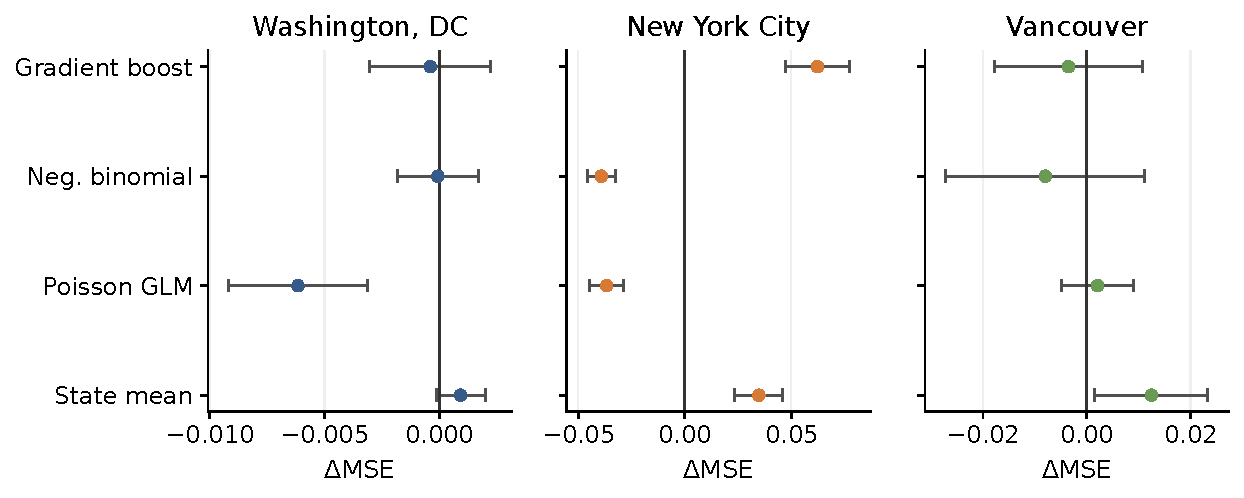
\includegraphics[width=\textwidth]{figures/e11/e06_mse_improvement.pdf}
\caption{Held-out integer-MSE change after adding lagged bicycle state.
Positive values favor the bicycle-aware specification; comparisons are
paired within city and model family.}
\label{fig:mse_improvement}
\end{figure}


\begin{table}[!htbp]
\caption{Matched held-out integer-prediction MSE, DELB, and Predictability Gap results for July--December 2022. The paired DELB column reports the baseline and bicycle-augmented lower bounds as \(L^0/L^B\). Positive \(\Delta\mathrm{MSE}\) denotes lower error after adding bicycle information. Gap narrowing is \(\Delta G=\Delta\mathrm{MSE}-\Delta L\): a positive value indicates that the model moved closer to the lower bound, whereas a negative value indicates that the estimated lower bound decreased more than the model MSE. Differences were calculated from unrounded values and then rounded for display.}
\label{tab:prediction_gap_results}
\begin{adjustwidth}{-\extralength}{0cm}
\raggedleft
\begin{tabular*}{\linewidth}{@{\extracolsep{\fill}}llrrrrrr@{}}
\toprule
\textbf{City} & \textbf{Model} & \(\boldsymbol{\mathrm{MSE}^0}\) &
\(\boldsymbol{\mathrm{MSE}^B}\) & \(\boldsymbol{L^0/L^B}\) &
\(\boldsymbol{\Delta\mathrm{MSE}}\) &
\(\boldsymbol{\Delta L}\) & \textbf{Gap narrowing}\\
\midrule
Washington, DC & State mean & \rev{0.5002} & \rev{0.4993} & 0.107/0.092 & \rev{0.0009} & 0.015 & -0.014\\
Washington, DC & Poisson GLM & \rev{0.4933} & \rev{0.4994} & 0.107/0.092 & \rev{-0.0062} & 0.015 & -0.021\\
Washington, DC & Negative-binomial GLM & \rev{0.4931} & \rev{0.4932} & 0.107/0.092 & \rev{-0.0001} & 0.015 & -0.015\\
Washington, DC & Poisson gradient boosting & \rev{0.4952} & \rev{0.4956} & 0.107/0.092 & \rev{-0.0004} & 0.015 & -0.016\\
New York City & State mean & \rev{2.0893} & \rev{2.0545} & 0.263/0.230 & \rev{0.0348} & 0.034 & 0.001\\
New York City & Poisson GLM & \rev{1.9043} & \rev{1.9410} & 0.263/0.230 & \rev{-0.0367} & 0.034 & -0.070\\
New York City & Negative-binomial GLM & \rev{1.9073} & \rev{1.9465} & 0.263/0.230 & \rev{-0.0392} & 0.034 & -0.073\\
New York City & Poisson gradient boosting & \rev{1.9010} & \rev{1.8388} & 0.263/0.230 & \rev{0.0623} & 0.034 & 0.029\\
Vancouver & State mean & \rev{1.6632} & \rev{1.6507} & 0.259/0.208 & \rev{0.0125} & 0.051 & -0.038\\
Vancouver & Poisson GLM & \rev{1.6287} & \rev{1.6266} & 0.259/0.208 & \rev{0.0021} & 0.051 & -0.049\\
Vancouver & Negative-binomial GLM & \rev{1.6138} & \rev{1.6218} & 0.259/0.208 & \rev{-0.0080} & 0.051 & -0.059\\
Vancouver & Poisson gradient boosting & \rev{1.6654} & \rev{1.6690} & 0.259/0.208 & \rev{-0.0035} & 0.051 & -0.054\\
\bottomrule
\end{tabular*}
\end{adjustwidth}
\end{table}


\begin{figure}[H]
\centering
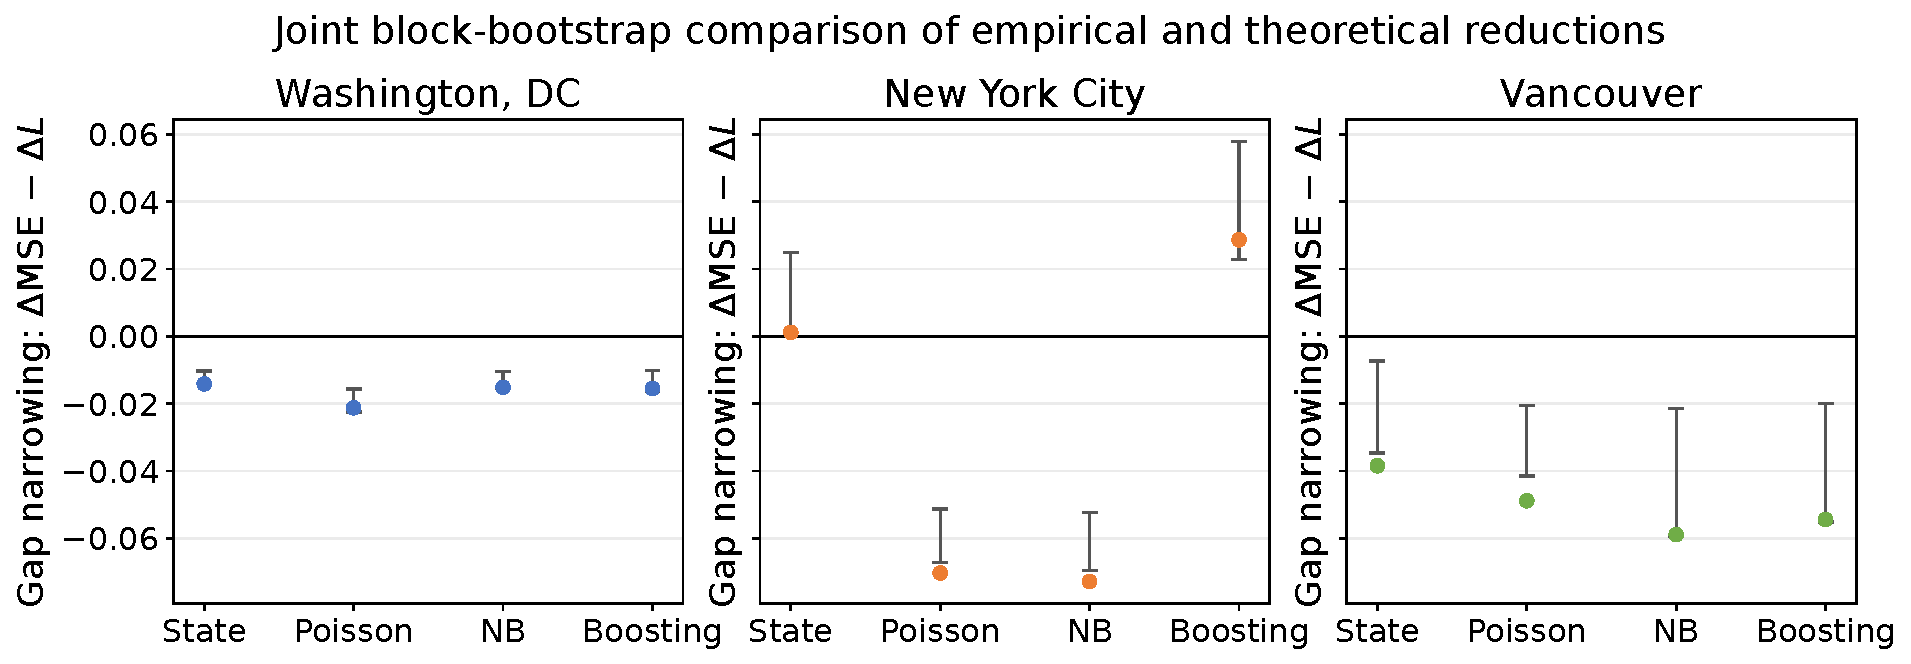
\includegraphics[width=\textwidth]{figures/e11/e07_gap_narrowing.pdf}
\caption{Predictability-gap narrowing after adding bicycle state. Positive
values mean empirical MSE fell by more than the estimated DELB; negative
values indicate a larger unused-information gap.}
\label{fig:gap_narrowing}
\end{figure}



\subsection{Secondary and Robustness Analyses}

\subsubsection{Fano Classification-Loss Comparison}
\label{subsec:results_fano}
All \FanoOracleRows{} population-oracle comparisons satisfied Fano's inequality,
and all empirical held-out modal-classifier errors remained above their
corresponding pretest Fano floors. No point-estimate violations
were observed.

Adding the bicycle state lowered the estimated Miller--Madow Fano floor
in all six city--target comparisons. Reductions ranged from \FanoFloorReductionMin{} to \FanoFloorReductionMax{}.
In contrast, held-out modal-classifier error increased in all six comparisons,
alongside increases in the number of unseen bicycle-augmented test states
(Table~\ref{tab:e14_fano_results} and Figure~\ref{fig:e14_fano}).

The opposite directions of the floor and classifier error are consistent
with the inequality. Added information can lower a population or pretest
error bound while sparse finite-sample state estimation worsens the
performance of a particular classifier. The Fano and DELB magnitudes are
not directly comparable because they concern different targets and loss
functions.




\begin{table}[!htbp]
\caption{\rev{Miller--Madow Fano floors and held-out statewise modal-classifier errors. The interval refers to the baseline-minus-bicycle floor reduction. The final column gives baseline/bicycle-aware counts of test observations assigned through the pretest global-mode fallback because their states were unseen before testing.}}
\label{tab:e14_fano_results}
\centering
\small
\setlength{\tabcolsep}{2.5pt}
\begin{tabular*}{\textwidth}{@{\extracolsep{\fill}}llccccc@{}}
\toprule
\textbf{City} & \textbf{Target} & \textbf{Base floor} & \textbf{Bike floor} & \textbf{Reduction [95\% CI]} & \textbf{Test error} & \shortstack{\textbf{Unseen test}\\\textbf{observations}}\\
\midrule
Washington, DC & Binary occurrence & 0.126 & 0.115 & 0.010 [0.010, 0.011] & 0.200/0.205 & 865/2,071\\
Washington, DC & Three-level count & 0.133 & 0.122 & 0.012 [0.011, 0.013] & 0.232/0.235 & 865/2,071\\
New York City & Binary occurrence & 0.150 & 0.124 & 0.027 [0.024, 0.029] & 0.358/0.364 & 2,058/4,408\\
New York City & Three-level count & 0.181 & 0.151 & 0.030 [0.027, 0.033] & 0.445/0.450 & 2,058/4,408\\
Vancouver & Binary occurrence & 0.200 & 0.175 & 0.025 [0.022, 0.028] & 0.326/0.335 & 234/812\\
Vancouver & Three-level count & 0.261 & 0.224 & 0.038 [0.034, 0.041] & 0.393/0.401 & 234/812\\
\bottomrule
\end{tabular*}
\end{table}


\begin{figure}[H]
\begin{adjustwidth}{-\extralength}{0cm}
\centering
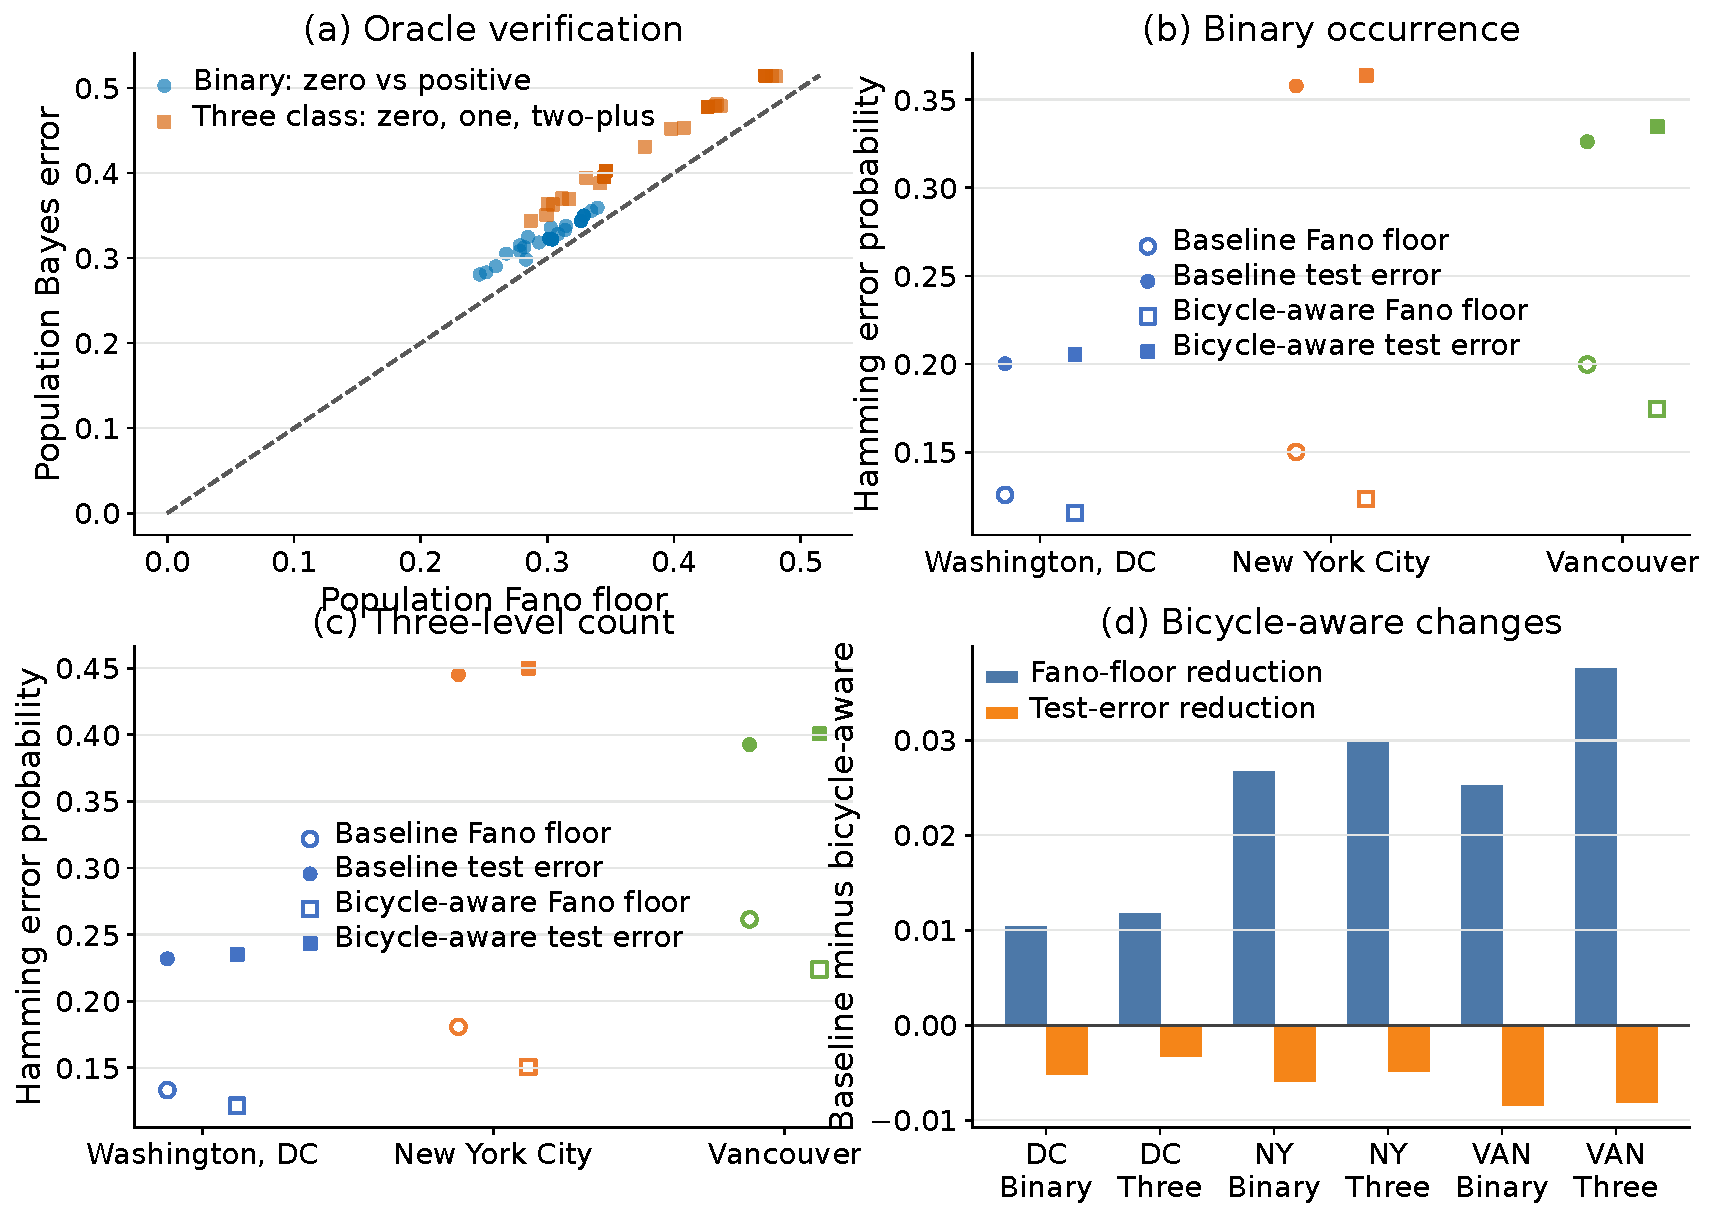
\includegraphics[width=\linewidth]{figures/s7/e14_fano_main.pdf}
\end{adjustwidth}
\caption{Fano classification-loss comparison. Oracle panels compare true
Bayes errors with true Fano floors; empirical panels compare estimated
pretest floors with held-out modal-classifier errors.}
\label{fig:e14_fano}
\end{figure}



\subsubsection{Crime-Type Heterogeneity}
\label{subsec:results_crime_types}

All \PositiveCrimeTypeTheory{} pooled city--category CMI estimates were positive.
Property theft produced the largest estimated DELB reduction in each city:
0.009 in Washington, DC, 0.045 in New York City, and 0.060 in Vancouver.
Vehicle theft and burglary produced smaller reductions
(Supplementary Materials, Section S4).

Four of the 36 matched city--crime-type--model comparisons passed the
adjusted positive-prediction screen, all in New York City. Only the
New York property-theft gradient-boosting model also narrowed the estimated
Predictability Gap. Because the primary randomization calibration was
not repeated within each crime category, these category-specific results
are treated as exploratory.



\subsubsection{Alternative Specifications and Rolling Origins}
\label{subsec:results_robustness}

The sign of the estimated DELB reduction was stable across the
prespecified theoretical alternatives. DELB reductions were positive in all
16 specifications in each city for the plug-in, Miller--Madow, and coherent
observed-support Jeffreys--Dirichlet estimators, including alternative
spatial and temporal resolutions, state mappings, estimators,
lag definitions, and bicycle-flow measures. Magnitudes across
aggregation levels are not directly comparable because the target
and MSE units change.

Rolling-origin prediction remained model- and city-dependent. New York
gradient boosting improved at all 12 monthly origins, with a mean MSE
reduction of 0.076, and the New York state-mean model improved at 11
origins, with a mean reduction of 0.030. The state-mean model improved
at eight origins in both Washington, DC and Vancouver, with mean
reductions of 0.001 and 0.006. Most GLM averages were negative. Complete
rolling-origin results are reported in Supplementary Materials, Section S5.

The alternative specifications therefore support the robustness of the
positive point-estimate pattern, while the rolling-origin results
show that conversion of the augmented state into improved prediction
depends on both city and model family.
